\section{Theorie}
\label{sec:Theorie}

Der Franck-Hertz-Versuch gehört zu den Elektronenstoßexperimenten, 
mit denen eine Strukturuntersuchung der Elektronenhüllen durchgeführt werden kann.
Die zu untersuchenden $\ce{Hg}$-Atome werden dafür mit Elektronen geeigneter Energie beschossen, 
wodurch elastische und inelastische Wechselwirkungen entstehen.
Im Falle eine inelastischen Stoßes wird das $\ce{Hg}$-Atom aus seinem Grundzustand der Energie $E_0$
in den ersten angeregten Zustand der Energie $E_1$ gehoben.
Für die Differenz dieser Energien gilt
\begin{equation}
    \frac{m_{0} \cdot v_{\text{vor}}^{2}}{2}-\frac{m_{0} \cdot v_{\text{nach}}^{2}}{2}=E_{1}-E_{0} \, ,
\end{equation}
mit der Ruhemasse $m_0$ und den Geschwindigkeiten $v_{\text{vor}}$ und $v_{\text{nach}}$ der Elektronen vor und nach dem Stoß.
Der damit beschriebene Energieverlust gibt Aufschluss über die Struktur der Elektronenverteilung.
Eine Energiebestimmung der angeregten $\ce{Hg}$-Atome erfolgt hierbei durch die Gegenfeldmethode.


\subsection{Aufbau des Frank-Hertz-Versuchs}\label{subsec:aufbau}

\begin{figure}
    \centering
    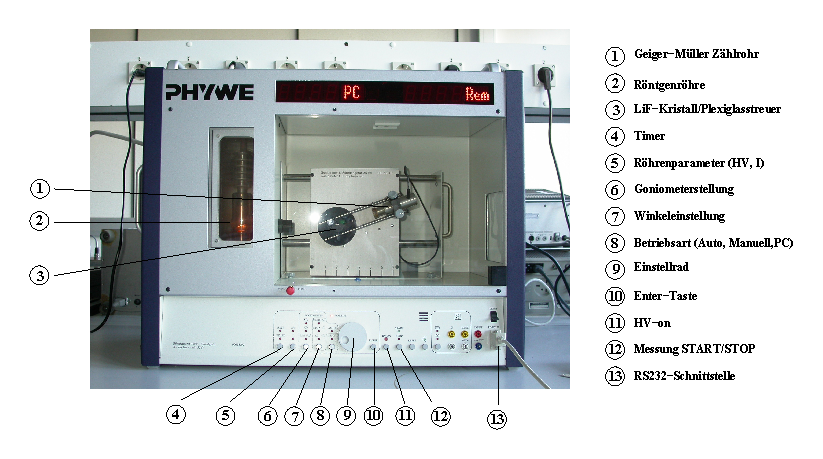
\includegraphics[width=0.6\linewidth]{pictures/aufbau.pdf}
    \caption{Prinzipieller Aufbau des Franck-Hertz-Versuchs. \cite{v601}}
    \label{fig:aufbau}
\end{figure}

In \autoref{fig:aufbau} ist der prinzipielle Aufbau des Versuchs dargestellt.
In dem evakuierten Gefäß befindet sich Quecksilber, welches gemäß der Dampfdruckkurve verdampft,
bis sich ein Gleichgewichtsdruck einstellt, welches von der Umgebungstemperatur $T$ abhängt.
Eine Regulation der Dampfdichte erfolgt also über die Temperatur $T$.
Innerhalb des Gefäßes wird ein Glühdraht aus Wolfram erhitzt, 
infolgedessen aufgrund des glühelektrischen Effekts Elektronen austreten.
Dem gegenüber befindet sich eine netzförmige Beschleunigungselektrode, an der die Spannung $U\text{B}$ liegt.
Nach Erreichen der Elektrode besitzen die beschleunigten Elektronen, die zuvor die Geschwindigkeit $v = 0$ hatten, die kinetische Energie
\begin{equation}
    \frac{m_{0} \cdot v_{\mathrm{vor}}^{2}}{2} = \mathrm{e}_{0} \, U_{\mathrm{B}} \, .
\end{equation}

Hinter der Beschleunigungselektrode befindet sich eine Auffängerelektrode, 
welche negativ geladen ist und die beschleunigten Elektronen abbremst.
Allein Elektronen, für deren Geschwindigkeit $v_\text{z}$ in Feldrichtung
\begin{equation}
    \frac{m_{0} \cdot v_{z}{ }^{2}}{2}  \geq \mathrm{e}_{0} \, U_{\mathrm{A}}
\end{equation}
gilt, erreichen die Auffängerelektrode während die anderen zur Beschleunigungselektrode zurückkehren.

Die sich im Beschleunigungsraum aufhaltenden $\ce{Hg}$-Atome wechselwirken nun mit den Elektronen auf unterschiedlichen Weisen.
Bei geringen Energien treten elastische Stöße auf. 
Aufgrund dem Massenverhältnis $m_0/M$ ergibt sich ein vernachlässigbarer Energieverlust von
\begin{equation}
    \increment E=\frac{4 \, m_{0} \, M}{\left(m_{0}+M\right)^{2}} \cdot E \approx \num{1.1e{-5}} \, E \, ,
\end{equation}
mit der Energie der Elektrons $E$. 
Dabei kommt es zu einer Richtungsänderung, welche zu beachten ist.

Haben die Elektronen eine Energie der Energiedifferenz $E_1 - E_0$ oder höher, kommt es zu inelastischen Stößen.
Auf die $\ce{Hg}$-Atome wird der Betrag der Energiedifferenz übertragen, wodurch sie angeregt werden während die restliche Energie die Elektronen behalten. 
Das $\ce{Hg}$-Atom geht vom ersten angeregten Zustand unter Emission einer elektromagnetischen Welle wieder in den Grundzustand über. 
Das emittierte Lichtquant besitzt eine Energie von
\begin{align}
    \text{h} \, \nu &= E_1 - E_0 \\
    \intertext{und damit eine Wellenlänge von}
    \lambda = \frac{h \cdot c}{E_1 - E_0}
\end{align}\begin{equation}
    \text{h} \, \nu = E_1 - E_0 \, 
\end{equation}
wobei h das Plancksche Wirkungsquantum und $\nu$ die Frequenz der emittierten Strahlung ist.

\begin{figure}[H]
    \centering
    \includegraphics[width=0.6\linewidth]{pictures/frank-hertz-kurve.pdf}
    \caption{Der Auffängerstrom $I_\text{A}$ in Abhängigkeit der Beschleunigungsspannung $U_\text{B}$. \cite{v601}}
    \label{fig:fhkurve}
\end{figure}

Die Gegenfeldmethode dient der Beobachtung des Stroms der Auffängerelektrode in Abhängigkeit der Beschleunigungsspannung,
wie es in \autoref{fig:fhkurve} dargestellt ist.
Sobald die Beschleunigungsspannung $U_\text{B}$ größer ist als die Spannung der Auffängerelektrode, wird ein schlagartig wachsender Strom registriert.
Nachdem die Elektronen eine Energie von $E_1 - E_0$ erreichen, wechselwirken sie mit den $\ce{Hg}$-Atomen inelastisch und sie verlieren ihre Energie.
Dies verursacht, dass sie die Auffängerelektrode nicht mehr erreichen und der Auffängerstrom $I_\text{A}$ plötzlich abnimmt.
Sobald die Beschleunigungsspannung erneut auf ein Niveau ansteigt, an dem die Elektronen den Energiebetrag der Energiedifferenz besitzen,
können sie im Beschleunigungsraum ein zweites Mal mit den $\ce{Hg}$-Atomen inelastisch stoßen.
Der Auffängerstrom $I_\text{A}$ wird in periodischen Intervallen der Länge $U_1$ immer wieder ansteigen und abrupt abfallen. 
Die Länge $U_1$ bezeichnet das erste Anregungspotential
\begin{equation}
    U_{1}:=\frac{\left(E_{1}-E_{0}\right)}{e_{0}} \, .
\end{equation}


\subsection{Einflüsse auf die Gestalt der Franck-Hertz-Kurve}

Die in \autoref{fig:fhkurve} dargestellte Franck-Hertz-Kurve weicht aufgrund von einigen Störeinflüssen signifikant ab, 
welche in dem Folgenden genannt werden sollen.


\subsubsection{Kontaktpotential}

Da die Elektroden aus Materialien bestehen, die eine unterschiedliche Austrittsarbeit der Elektronen besitzen,
weicht das tatsächliche Beschleunigungspotential von der, die angelegten ist ab.
Hierbei ist die Austrittsarbeit des Glühdrahts $\Phi_\text{G}$ als die Austrittsarbeit der Beschleunigungselektrode $\Phi_\text{B}$,
weswegen das Beschleunigungspotential verschoben ist. Diese Potentialverhältnisse sind in \autoref{fig:kontakt} dargestellt.
\begin{figure}
    \centering
    \includegraphics[width=0.8\linewidth]{pictures/kontakt.pdf}
    \caption{Potentialverhältnisse zwischen Glühkathode und Beschleunigungselektrode. \cite{v601}}
    \label{fig:kontakt}
\end{figure}
Das tatsächliche Beschleunigungspotential $U_\text{B, eff}$ hat den Wert
\begin{align}
    U_\text{B, eff} = U_\text{B} K \\
    \intertext{mit dem Kontaktpotential}
    K = \frac{\left( \Phi_\text{B} - \Phi_\text{G} \right)}{e_0} \label{eq:Kontaktpotential}
\end{align}
Die Franck-Hertz-Kurve ist also um den Wert K verschoben.


\subsubsection{Energie-Spektrum der Elektronen}

Die durch den glühelektrischen Effekt emittierten Elektronen folgen keiner diskreten Energieverteilung,
da sie bereits im Inneren des Metalls ein Energie-Spektrum besitzen, welches Fermi-Dirac-Verteilung genannt wird.
Aus diesem Grund treten die Elektronen bei der Glühemission mit unterschiedlichen Anfangsgeschwindigkeiten aus
und besitzen beim Durchlaufen des Beschleunigungspotentials $U_\text{b, eff}$ ein Energie-Spektrum,
welches hin zu höheren Energien abnimmt.
Somit treten die inelastischen Stöße in einem endlichen Spannungsbereich auf.
Die Franck-Hertz-Kurve wird daher ihren Anstieg in der Nähe eines Maximums verringern 
und danach nicht mehr unstetig auf Null abfallen, sondern sich stetig dem Stromminimum nähern.


\subsubsection{Elastische Wechselwirkungen}

Die in \autoref{subsec:aufbau} erwähnten Richtungsänderung, die aufgrund von elastischen Stößen auftreten,
führen zu keinen merklichen Energieabnahmen der Elektronen. 
Sie verändern daher die Gestalt der Kurve nicht wesentlich, solange sie innerhalb des Beschleunigungsraumes geschehen.
Treten sie jedoch zwischen Beschleunigungs- und Auffängerelektrode auf, führen sie zu einer Verteilung der z-Komponente der Geschwindigkeiten.
Aufgrund der $v_\text{z}$-Abhängigkeit im Gegenfeld, führt dieser Einfluss zu einer Abflachung und VErbeiterung der Franck-Hertz-Kurve.


\subsubsection{Dampfdruck}

In einem bestimmten Dampfdruckbereich kommt es zu einer erwarteten Anzahl Wechselwirkungen.
Damit diese in messbaren Maßen auftreten, muss die mittlere freie Weglänge $\bar{w}$ der Atome klein im Vergleich
zum Abstand $a$ zwischen Kathode und Beschleunigungselektrode sein. 
Ist der Dampfdruckbereich klein, kann es auch bei sehr großer Bremsspannung $U_\text{B}$ nur vereinzelt zu Anregungen kommen, 
da die Stoßwahrscheinlichkeit klein ist. 
Bei sehr hohen Dampfdruckbereichen spielt der Energieverlust der elastischen Stöße eine immer größere Rolle, 
da es viel häufiger Stößen kommt.

Mithilfe des Sättigungsdrucks $p_\text{sät}$ kann die mittlere freie Weglänge zu
\begin{equation}
    \bar{w} \, [\unit{\centi\meter}] = \frac{0.0029}{p_\text{sät}} \, \left[ \frac{1}{\unit{\milli\bar}}\right]
\end{equation}
bestimmt werden.
Da der Sättigungsdruck temperaturabhängig ist, ergibt sich für $\ce{Hg}$ 
\begin{equation}
    p_\text{sät}(T) = \num{5.5e7} \exp{\left( \frac{-6876}{T} \right)} \, .
\end{equation}